\documentclass[../main.tex]{subfile}
\begin{document}
 \normalsize
\section{Theoretical Background}
In order to describe the superconductors we are going the introduce the second quantisation formalism.
It allows us to describe the wavefunction of a system using creation and anihinaltion operators over
energystates of the system and simplify a lot the notation. The mathematical fundation of this formalism
lays in the Hilbert space, its dual space and furthermore we are going to introduce the Foch space.\\

It's also relevant for our study that we are going to work on fermions. The formalism stays the same for 
bosons but the results are fundamentaly different. One can mention the Pauli principle as an exemple which
only applies on fermion is can be derived with the help of the second quantisation.\\ 

\subsection{Bosons and fermions}
We consider without loss of generality the following hamiltonian. 
\begin{equation}\label{eq:MasterHamiltonian}
    \hat{H} = \hat{H}_0 + \hat{H}_I
\end{equation}
with the single particle operator $\hat{H}_0$ and the interaction operator $\hat{H}_I$:
\[
    \hat{H}_0 = \sum_{i\in \natset{N}} \hat{h}_i(x_i)~,~~ \hat{h}_i(x_i) = -\frac{\hbar^2}{2m}\nabla_i^2 + \hat{U}(x_i)
\]
Where we introduce the notation $\natset{N} = \{n \in \mathbb{N}: n\leq N\}$. We call it single particle operator 
because the operator only applies on a particle. It may depend from the particle's postion $\bm{r}$ or spin $s$: 
$x_i := (\bm{r}, s) \in \mathcal{X}\subseteq\mathbb{R}^{3}\times\mathbb{S}$. For exemple we have for an electron 
$\mathbb{S}= {-\frac{1}{2},\frac{1}{2}}$ A single particle operator is in this case the sum of the kinetic- 
and potential energy operators.\\

Further we describe a quantum state that a particle can occupy with a wavefunction $\phi_{\nu}(x)$, 
which own a certain energy $\epsilon_n \in\mathbb{R}$. This energy depends on 
the wavevector and the spin of the particle: $\nu = (\bm{k}, \sigma)$. The fundamental equation of
quantum mechanics relates the wave function with the hamiltonian using the energy of the state:
\[
    \hat{h} \phi_{\nu}(x) = \epsilon_\nu \phi_{\nu}(x)
\]
The wave function lay in the Hilbert space [more details?]. Therefor $\phi_{\nu}(x)$ are eigenfunction or -states of
the Hamiltonian with eigenvalues $\epsilon_{\nu}$. Further the wavefunction should build an orthonormal basis:
\[
    \int_\mathcal{X} \phi_{\nu'}(x) \phi_{\nu}(x) \dd x = \delta_{\nu'\nu}.
\]
$\nu$ and $\nu'$ are two different states. We introduced here the korenker delta $\delta_{\nu'\nu}$ which is one when the two indicies
are equal and zero otherwise. Because the spin $s$ is not continuous one can understand the integral in the following way:
\[
    \int_\mathcal{X} \dd x = \sum_{s\in \mathbb{S}} \int_{\mathbb{R}^3} \dd^3 r
\]  
where $ \int_{\mathbb{R}^3}\dd r^3 = \int_{\mathbb{R}}\int_{\mathbb{R}}\int_{\mathbb{R}} \dd r_1 \dd r_2 \dd r_3$.
We integrate over all possible states.\\

Now that we can describe one particle we want to describe a system containing many instance of that particle.
The wavefunction sums up all possible combination of wavefunction in the system and should stay normalsized. 
A combination is discribed as the product of the wavefunction of the particle in a certain state. These particle
can be swaped and therfore we need to consider all combinations.
 We restrict ourselves to fermions and bosons. We admit having $N \in \mathbb{N}$ paricles in the system.\\

\paragraph{Bosons}
The many-particle wavefunction of the bosons is a symetric (exponent $S$) under swap of two particles.
\[
    \Phi^{(S)}(x_1,..,x_N) = \left(N!\prod_{N}(n_{\nu})!\right)^{-\frac{1}{2}} \sum_{P\in S_n} P \phi_{\nu_1}(x_1)\cdot ..\cdot \phi_{\nu_N}(x_N)
\]
This represents the an eigenfunction of the non interacting bosonic-Hamiltonian.
We used $n_{\nu}$, which represents the number of particle in the state $\nu$. Therefor we usaly call it the occupation number of the state $\nu$.
For fermion this integer has no constrain in general.
The permutation set $S_n$ contains all the possbile combinations of $x_i$ in the state $\nu_j$ for $i,j\in\natset{N}$.

\paragraph{Fermions}
Fermions are a bit different, their many-particle fermion wavefunction is antisymmetric under swap of two particles. We denote it as
\[
    \Phi^{(A)}(x_1,..,x_N) = \left(N!\right)^{-\frac{1}{2}} \sum_{P\in S_n} \signum{P}\cdot P \phi_{\nu_1}(x_1)\cdot ..\cdot \phi_{\nu_N}(x_N).
\]
which is an eigenfunction of the non interacting fermionic-Hamiltonian.
$\text{sgn}$ represents the signum function. Applied on a permutation $P$ it is one if $P$ is even and minus one if $P$ is even.\\
We already know that the Pauli principle implies that it can be up to one particle in each energy state. We therfore have $n_\nu \in \{0,1\}$. The normalsization
factor is the same but the product over the ones vanishes.\\

At this point one might have recognised the formula of the determinant
\[
    \Phi^{(A)}(x_1,..,x_N) = \left(N!\right)^{-\frac{1}{2}} \text{det}\begin{pmatrix}
        \varphi_{\nu_1}(x_1)& \cdot\cdot &\varphi_{\nu_1}(x_N)\\
        \vdots&  &\vdots\\
        \varphi_{\nu_N}(x_1)& \cdot\cdot &\varphi_{\nu_N}(x_N)\\

    \end{pmatrix},
\]
which vanishes if two rows or columms are identic. We usaly describe this expression as the Slatter determinant. This means that the probability of finding two fermions in the same state is zero.
This is the Pauli principle. Only one or no particle may occupy each state.\\

Further we entcounter a major problem. The many-particle wave function of fermions is defined up to a sign. For instance if we consider
two particles ``having'' $x_1$ and $x_2$, we have two possible state $\nu_1$ and $\nu_2$. To possible soltutuion are
\begin{align*}
    &\Phi^{(A_1)} = \frac{1}{\sqrt{2}} \bigl(\varphi_{\nu_1} (x_1)\varphi_{\nu_2} (x_2) - \varphi_{\nu_1} (x_2)\varphi_{\nu_2} (x_1) \bigr)\\
    \text{or~} &\Phi^{(A_2)} = \frac{1}{\sqrt{2}} \bigl(\varphi_{\nu_1} (x_2)\varphi_{\nu_2}(x_1) - \varphi_{\nu_1} (x_1)\varphi_{\nu_2} (x_2)\bigr)\\
    &~~~~~~~=-\Phi^{(A_1)}.
\end{align*}
This sign difference may lead to computation errors. We aim to give a labeling to our states when we count them and keep it when it 
comes to build the Slatter determinant.\\

These bosonic and fermionic wavefunctions are eigenstate of the Hamiltonian $\hat{H}_0$ and the corresponding eigenvalue $E_{\nu}$
is given by summing the energy of each state times its occupation number: $E_{\nu} = \sum_{\nu} \epsilon_{\nu} n_{\nu}$.
For this reason it's important that they build an orthonormal basis:
\[
    \int_{\mathcal{X}^N} \Phi_a^{\ast}(x_1,..,x_N) \Phi_b(x_1,..,x_N) \dd^N x = \delta_{ab}.
\]
Therfore we can expend any many-particle wavefunction $\Psi$ as the linear combination of these:
\[
    \Psi = \sum_a f_a \Phi_a(x_1,..,x_N)
\]
where $f_a$ is a coefficent and $a$ a labeling.\\

What we just discused is the so called first quantisation- or wave function formalism. Now we intend to introduce a better way of 
describing our system.

\subsection{The second quantisation}
For a better description of the many-particle system we introduce a simpler notation. The second quantisation lays on three important objects. States described as ``ket''. We put any relevant information between the ket
e.g. $|\bm{k}, \sigma,..\rangle$. Then we need operators that act on these states to allow interactions in the system. 
We need an operator that creates a states and another that anihilates a state.\\

\paragraph{States} In this section we describe a state as the number of particle that occupies each single-particle state. Therfore
we order the state $1<2<..<N$. We then can describe the wave function as follow $|n_{1},..,n_{N}\rangle$.\\

Further the state where no particle are present is called the vaccum state and we denote it as $|0_{\nu_1},..,0_{\nu_N}\rangle = |0\rangle$.

\subsubsection{Second quantisation for fermions}
\paragraph{Creation operator $c_\nu^{\dagger}$}
The creation operatortor adds a particle in the state that is concernd and rephase the state:
\[
    c_{\nu}^{\dagger} |n_{1},..,n_{\nu},..\rangle = (-1)^{\sum_{\mu<\nu}n_{\mu}} (1-n_{\nu})|n_{1},..,n_{\nu}+1,..\rangle
\]
We notice the $ (1-n_{\nu})$ term which avoid to create a particle at the state, if one already exist. This is the expression of
the Pauli-principle. 
and we can then construct a state by appling this operator after another on the vaccum state. To avoid the minus one to add a negative sign, we start from the 
end and add the particle backwards in the order of the state:
\[
    |n_{1},..,n_{N}\rangle = (c_{1}^{\dagger})^{n_{1}}\cdot ..\cdot (c_{N}^{\dagger})^{n_{N}} |0\rangle
\]  

\paragraph{Annihilation operator $c_\nu$}
Likewise the anihinaltion operator destroys a particle in the corresponding state. The operator reads
\[
    c_{\nu}^{\dagger} |n_{1},..,n_{\nu},..\rangle = (-1)^{\sum_{\mu<\nu}n_{\mu}} (n_{\nu})|n_{1},..,n_{\nu}-1,..\rangle.
\]
We can easly recognise that due to the $n_{\nu}$-term, destroying a particle that doesn't exist gives zero, 
so it's only possible to destroy particle that exist. Further we intend to introduce some few compution 
rules that are going to help us later. \\

The anticommutator of two operator reads $[A,B]_{+}$ or $\{A,B\} := AB + BA$ and is an opertor as well.
We're going to stick with $[A,B]_{+}$ since it's more consitent with the commutatotor notation $[A,B]_{-}$ (or simply $[A,B]$).\\

The follwoing results are obtain by separting the $\nu = \mu$ from the $\nu \neq \mu$. We must also say that the dagger $\dagger$ 
should be understand as the complex transpose of the operator and $(AB)^{\dagger} = B^{\dagger}A^{\dagger}$.
\begin{align}
    [c_{\nu},c_{\mu}]_+ =&~ 0 \label{eq:Fermion1} \tag{$\mathfrak{Fer}_1$}\\
    [c^{\dagger}_{\nu},c^{\dagger}_{\mu}]_+ =&~0 \label{eq:Fermion2} \tag{$\mathfrak{Fer}_2$}\\
    [c^{\dagger}_{\nu},c_{\mu}]_+ =&~ \delta_{\mu,\nu}\label{eq:Fermion3} \tag{$\mathfrak{Fer}_3$}
\end{align} 

We can then combine the creation and anihinaltion operator to count the number of particles in a state:
\[
    c_{\nu}^{\dagger} c_{\nu} |n_{1},..,n_{\nu},..\rangle = n_{\nu}|n_{1},..,n_{\nu},..\rangle.
\]  
From this we can define the number operator $\hat{n}_{\nu}:= c_{\nu}^{\dagger} c_{\nu}$ which we can combine in the total number operator
\[
    \hat{N} = \sum_{\nu} \hat{n}_{\nu}~,~~\text{where logicaly}~ N = \sum_{\nu} n_{\nu}
\]
if we apply the operator on a state.\\

\paragraph{Second quantisation description of the single- and two- particle operators}
We first need to make an important observation between the Slatter determinant and the single particle state to
understand the following. First we introduce two basis element |$\Phi_{\alpha}\rangle$ and $|\Phi_{\beta}\rangle$, which can be many-particles eigenstate of the system.
We can also call them Slatter determinant.
Further we introduce the probability of the configuration $|\Phi_{\alpha}\rangle$ to scatter into the $|\Phi_{\beta}\rangle$ due to the action of an operator $A$ (momentum, potental, interactions,..).
This is described by the matrix element $\langle\Phi_{\alpha}|A|\Phi_{\beta}\rangle$ which involves the single particle states $|\alpha_1\rangle, .., |\alpha_N\rangle$ of $|\Phi_{\alpha}\rangle$
and $|\beta_1\rangle, ..,|\beta_N\rangle$ of $|\Phi_{\beta}\rangle$.
\[
    \langle\Phi_{\alpha}|A|\Phi_{\beta}\rangle = \sum_{i,j} C_{ij}\langle\alpha_i|A|\beta_j\rangle
\]
involving some constants $C_{ij}$. This describes the overlapp of the two configurations, after that we modified $|\Phi_{\beta}\rangle$ with $A$.
On the right hand side (r.h.s) we introduced the braket scalar product notation. The bra $\langle\alpha|$ lives in the dual space
of the Hilbert space. One reads it as the complexe transpose of $|\alpha\rangle$.\\

We recall the single particle Hamiltonian we introduced earlyer. Its second quantisation representation reads
\begin{equation}\label{eq:SecondQuantisationSingleParticle}
    \hat{H}_0 = \sum_{i \in \natset{N}} \hat{h}(x_i) ~ \leadsto ~~ \sum_{\alpha,\beta} \langle \alpha|\hat{h}|\beta\rangle c_{\alpha}^{\dagger}c_{\beta}
\end{equation}
where $\alpha$ and $\beta$ are single-particle states of the system. $c_{\alpha}^{\dagger}c_{\beta}$ tries to transfert a fermion
from the state $|\beta\rangle$ to the state $|\alpha\rangle$.
We have
\begin{equation}\label{eq:Translation_TwoStateOverlap}  
    \langle \alpha|\hat{h}|\beta\rangle = \int  \varphi_{\alpha}^{\ast}(x) \hat{h}(x) \varphi_{\beta}(x) \dd x\\
\end{equation}
where $x$ still represents the position and the spin of the particle.\\
$\hat{h}$ is a single particle operator, it means it acts on one particle at a time.
Two states are going to be changed. $|\alpha\rangle$ loses a particle and $|\beta\rangle$ gains one. We say for instance, that the 
configuration before the scattering is $|\Phi\rangle$ and after the scattering is $|\Phi'\rangle$. 
This means, if our two slatter determinant $|\Phi\rangle$ and $|\Phi'\rangle$ differs in more than two state, there are
some scattering that we can't describe, so the overlapp must be zero. We allow only two states to be modified. Otherwise the single-particle
states differ and due to their orthonal properties, we get a zero.\\

Similarly for the two-particle operator we have
\begin{equation}\label{eq:SecondQuantisationDoubleParticle}
    \hat{H}_I = \frac{1}{2}\sum_{i\neq j \in \natset{N}} \hat{v}(x_i, x_j) ~ \leadsto ~~ \frac{1}{2}\sum_{\alpha,\beta,\gamma,\delta} \langle \alpha\beta|\hat{v}|\gamma\delta\rangle c_{\alpha}^{\dagger}c_{\beta}^{\dagger}c_{\gamma}c_{\delta}
\end{equation}
involving a more nested overlap of the four states:
\begin{equation}\label{eq:Translation_FourStateOverlap}
    \langle\alpha\beta|\hat{v}|\gamma\delta\rangle = \int \int \varphi_{\alpha}^{\ast}(x) \varphi_{\beta}^{\ast}(x') \hat{v}(x,x') \varphi_{\gamma}(x) \varphi_{\delta}(x') \dd x \dd x'.
\end{equation}
which modifies four states so the overlapp of two slatter determinant vanishes if the determinant differ in at least four states.\\ 

The l.h.s of the equation is the matrix element $\langle\Phi_{\alpha}|\hat{v}|\Phi_{\beta}\rangle$ of the the operator
 $\hat{v}$, which involves two basis state |$\Phi_{\alpha}\rangle$ and $|\Phi_{\beta}\rangle$ .
On the r.h.s we have a description with wavefunctions, which own to the first quantisation. What we have here
is the bridge between the first and the second quantisation. One could compute each side separately and notice
that both formalism lead to the same result.

\subsubsection{Second quantisation for bosons}
\subsection{Basis transformation}
Until now considerd the wavefunction in a restricted basis $\{\varphi_{\alpha}(x)\}$. A wave function is defined as the overlapp between the basis and the state:
\[
    \phi(x) = \langle x | \alpha \rangle.
\]
Let us now define a more general new operator that create a states $|\alpha\rangle = a_{\alpha}|0\rangle$ for fermion and bosons.
We asume that we have another basis $\{|\tilde{\alpha}\rangle\}$.
We now want to show, that the new operator $a_{\alpha}$ can be expressed as a linear combination of the other operator  $a_{\tilde{\alpha}}$. This will be a
usefull too to jump from a basis to another. We first notice the following identity relations:
\[
    \mathbb{I} = \sum_{\alpha} | \alpha \rangle \langle \alpha| = \sum_{\tilde{\alpha}} | \tilde{\alpha} \rangle \langle \tilde{\alpha}| 
\]
this allow us to write 
\begin{align*}  
    a_{\alpha}^{\dagger}|0\rangle &= | \alpha \rangle = \sum_{\tilde{\alpha}}|\tilde{\alpha}\rangle\underbrace{\langle\tilde{\alpha}|\alpha\rangle}_{\text{scalar}} = \sum_{\tilde{\alpha}}\langle\tilde{\alpha}|\alpha\rangle |\tilde{\alpha}\rangle \\
\end{align*}
inverting the indicies leads to the same result, which leads to the transformation rules
\begin{align*}
    a_{\alpha}^{\dagger} &= \sum_{\tilde{\alpha}}\langle\tilde{\alpha}|\alpha\rangle a_{\tilde{\alpha}}^{\dagger}\\
    a_{\alpha} &= \sum_{\tilde{\alpha}}\langle\alpha|\tilde{\alpha}\rangle a_{\tilde{\alpha}}.
\end{align*}
Further we can use these relations to express a wavefunction in the basis of another wavefunction. We have
\begin{align*}
    \phi_{\alpha}(x) = \langle x|\alpha\rangle &= \langle x|\left(\sum_{\tilde{\alpha}} \langle \tilde{\alpha}|\alpha\rangle |\tilde{\alpha}\rangle\right) = \sum_{\tilde{\alpha}}  \langle \tilde{\alpha}|\alpha\rangle\langle x|\tilde{\alpha}\rangle
    = \sum_{\tilde{\alpha}} \langle \tilde{\alpha}|\alpha\rangle \varphi_{\tilde{\alpha}}(x).
\end{align*}
Inverting $\alpha$ and $\tilde{\alpha}$ leads as well $\varphi_{\tilde{\alpha}}(x) = \sum_{\alpha} \langle \alpha|\tilde{\alpha}\rangle \phi_{\alpha}(x)$.\\

Morover we can show that the basis transformation is unitary. This is an important feature because we can simplify the calculation by changing the basis but
the result we seek for would remain the same after the unitary transformation. Such transformations plays a major role later in the thesis.
We can save the $\langle \tilde{\alpha} | \alpha\rangle$ in a matrix $D$ and prove that this matrix is unitary. We have
\begin{align*}
    \langle \tilde{\alpha} | \tilde{\beta}\rangle  &= \sum_{\gamma} \langle \tilde{\alpha}|\gamma\rangle\langle \gamma | \beta\rangle =  \sum_{\gamma} \langle \tilde{\alpha}|\gamma\rangle \langle \beta | \gamma\rangle^{\ast}\\
    &=\sum_{\gamma} D_{\alpha\gamma}D_{\beta\gamma}^{\ast} = \sum_{\gamma} D_{\alpha\gamma}D^{\dagger}_{\gamma\beta} = (DD^{\dagger})_{\alpha\beta}.
\end{align*} 
meanwhile $\langle \tilde{\alpha} | \tilde{\beta}\rangle = \delta_{\tilde{\alpha} \tilde{\beta}}$ so that $DD^{\dagger} = \mathbb{I}$. The matrix $D$ is therfore unitary. \rem{
    but do we also have the orthonormality of if we take two different basis?}.\\

The last important step is to show that the basis transformation keeps the anti-, commutation relations. Let us for the seek of readability
use the notation $[A,B]_{\xi} = AB + \xi BA$ where $\xi = -$ for bosons and $\xi = +$ for fermions. We have for exemple using $[a_{\alpha}, a_{\alpha'}^{\dagger}]_{\xi} = \delta_{\alpha\alpha'}$
\[
    [a_{\tilde{\alpha}}, a_{\tilde{\alpha}'}^{\dagger}]_{\xi} = \sum_{\tilde{\alpha}\tilde{\alpha}'} \langle \tilde{\alpha}|\alpha\rangle\langle\alpha'|\tilde{\alpha}'\rangle [a_{\alpha}, a_{\alpha'}^{\dagger}]_{\xi} = \langle \tilde{\alpha}|\tilde{\alpha}'\rangle = \delta_{\tilde{\alpha}\tilde{\alpha}'}.
\]
The first step follows after spliting the commutator in two parts, insert the transformation and recombine the new commutator. 
The last step involves the orthonormality of the basis.
On the same way one can prove $[a_{\tilde{\alpha}},a_{\tilde{\alpha}'}] = [a_{\tilde{\alpha}}^{\dagger},a_{\tilde{\alpha}'}^{\dagger}] = 0$.
  
\subsubsection{Field operators}
Later in this thesis we are going to use field opertors to describe an order parameter of a superconductive system. These are 
creation and annihilation operators that are defined in the $|x\rangle$-space-spin basis regarding antoher basis $\{|\alpha\rangle\}$. We here give the state as an argument
an not as an index anymore. Despite the notation the following operators musn't be confused with a wavefunction.
\begin{align}
    \hat{\psi}^{\dagger}(x) &= \sum_{\alpha} \langle\alpha|x\rangle a_{\alpha}^{\dagger} = \sum_{\alpha} \varphi_{\alpha}^{\ast}(x) a_{\alpha}^{\dagger} \label{eq:FieldOp}\\ 
    \hat{\psi}(x) &= \sum_{\alpha} \langle\alpha|x\rangle a_{\alpha} = \sum_{\alpha} \varphi_{\alpha}(x) a_{\alpha}^{\dagger}\label{eq:FieldOpDag}
\end{align}
involving fermonic or bosonic operators $a$. We can then annihilation and create a particle at a spin-space location $x$. Beacause these operators
are involded, the commutations property respects which particle we are describing. Using the result we had for $[a_{\alpha}, a_{\alpha'}]_{\xi},
[a_{\alpha}, a_{\alpha'}^{\dagger}]_{\xi}$ and $[a_{\alpha}^{\dagger}, a_{\alpha'}^{\dagger}]_{\xi}$ where $\xi = -$ for the bosons and $+$ for the fermions. We find the following commutation relations:
\begin{align*}
    \left[\hat{\psi}(x), \hat{\psi}(x')\right]_{\xi} = & \left[\hat{\psi}(x)^{\dagger}, \hat{\psi}^{\dagger}(x)\right]_{\xi} = 0 \\
    \left[\hat{\psi}(x), \hat{\psi}^{\dagger}(x')\right]_{\xi} = &~ \delta(x-x')
\end{align*}
In the last expression we obtain a $\langle x | x '\rangle$ which cant normalsize the $\{|x\rangle\}$-basis so instead of a Korenker delta $\delta_{xx'}$
we get a delta distribution $\delta(x-x')$.
The goal is now to describe the Hamiltonian using this fields operators. Thefore we rebuild the fields operator in the Hamiltonian using a $\{|x\rangle\}$ basis
\begin{align*}
    \hat{H}_0 &=  \int \hat{\psi}^{\dagger}(x) \hat{h}(x)\hat{\psi}(x) \dd x\\
    \hat{H}_I &= \frac{1}{2} \int \int  \hat{\psi}^{\dagger}(x) \hat{\psi}^{\dagger}(x') \hat{v}(x,x')\hat{\psi}(x') \hat{\psi}(x) \dd x' \dd x
\end{align*}
We already know that the first and second quantisation are equivalent. We could now insert the definition of the field operators \ref{eq:FieldOp} and \ref{eq:FieldOpDag}
in the Hamiltonian and obtain a wave function description. Then we can just use the first to second quantisation translation \ref{eq:Translation_TwoStateOverlap} and \ref{eq:Translation_FourStateOverlap}
to a the second quantised representation. The reulst is a generlisation of the experession with the operators $a$.\\


\subsection{Interactive electron gas}
As we are later going to study, the electron are allowed to interact with each other. During such processes a photon is
usaly carying the momentum transfert of the scattering. We're going to use the formalism we introduced to 
find a second quantisation representation of the interacting Hamiltonian.\\

The system we're stying is a cube of side length $L$ with wolume $\Omega = L^3$ with $N$ electrons. Further we consider a periodic boundary condition for an arbitrary 
position vector $\bm{r} = (x,y,z)$:
\[
    (L,y,z) = (0,y,z)~,~(x,L,z) = (x,0,z)~,~(x,y,L) = (x,y,0).
\]  
We use the general form of the Hamiltonian \ref{eq:MasterHamiltonian} introduced in the beggining. We have a Coulomb potential and a kinetic energy term.
\begin{align}
    H_0 &= T+U =- \sum_{i\in \natset{N}} \frac{\hbar^2}{2m}\nabla_i^2 + \sum_{i\in \natset{N}} u(x_i)\\
    H_I &= V= \sum_{i\neq j \in \natset{N}} v(x_i, x_j)
\end{align} 
Where the pairwise potential is just a Coulomb potential $v(x_i, x_j) = \frac{e^2}{4\pi\epsilon_0|x_i - x_j|} = v(|x_i - x_j|)$.\\
\rem{drop of the hat?} We aim to describe the Hamiltonian in the momentum space, which is more convenient for the second quantisation. Therfore we first
need to find an expression for the wavevector $\bm{k}$. We describe a state $\alpha = (\bm{k}, \sigma)$ at a spin-space coordinate $x = (\bm{r}, s)$. First we take a plane wave solution of the Schrödinger equation:
\[
    \psi_{\bm{k}}(\bm{r}) = \frac{1}{\sqrt{\Omega}} e^{\im \bm{k}\cdot\bm{r}} \chi_\sigma(s)
\]
The periodicity of the system allows us to write $\psi(x=0) = \psi(x=L)$ using the boundary condition and obtain 
$1= e^{\im k_x L}$ as well as for the two other coordinates. The results reflects in the wavevector $\bm{k}$:
\[
    \bm{k} = \frac{2\pi}{L}(n_x, n_y, n_z)~,~~n_i\in \mathbb{Z}.
\]
As we saw earlier the eigenfunctions build a complete basis:
\begin{align*}
    \int \psi^{\ast}_{\alpha'}(x) \psi_{\alpha}(x) \dd x &= \int \sum_{s} \psi^{\ast}_{\alpha'}(x) \psi_{\alpha}(x) \dd x \\
    &=\frac{1}{\Omega} \int e^{\im\bm{r}\left(\bm{k}- \bm{k}'\right)} \underbrace{\sum_s \delta_{s\sigma}\delta_{s\sigma'}}_{\delta_{\sigma\sigma'}} \dd x\\
    &= \delta_{\bm{k}\bm{k}'}\delta_{\sigma\sigma'} = \delta_{\alpha\alpha'}.
\end{align*}    
where the integaral over the exponential function diverges if $\bm{k} \neq \bm{k}'$ so we use the case $\bm{k} = \bm{k}'$ and the integaral is zero otherwise.

The kinetic energy operator is a single particle operator so we have according to \ref{eq:SecondQuantisationSingleParticle} we have:
\[
    T = \sum_{\alpha,\alpha'} \langle \alpha|\frac{\hat{\bm{p}}^2}{2m}|\alpha'\rangle c_{\alpha}^{\dagger}c_{\alpha'}.
\]
Now we can juste use $\hat{\bm{p}} = \im \hbar \nabla$ and to compute this expression we use its 
first quantised form (see \ref{eq:Translation_TwoStateOverlap}) indvolving the $\delta_{\sigma\sigma'}$ trick we introduced
in the derivation of the complete basis. We also use  $\bm{k}' = \bm{k}$ and hide the $\frac{1}{\Omega}$ is the $\delta_{\bm{k}\bm{k}'}$. The result is
\[
T = \sum_{\alpha,\alpha'} \delta_{\alpha\alpha'} \frac{\hbar \bm{k}^2}{2m} c_{\alpha'}^{\dagger} c_{\alpha} = \sum_{\alpha} \underbrace{\frac{\hbar \bm{k}^2}{2m}}_{=:\epsilon_{\bm{k}}} c_{\alpha}^{\dagger} c_{\alpha}
\]
we recognise the occupation number operator $\hat{n}_{\alpha} = c_{\alpha}^{\dagger} c_{\alpha}$ and the energy of the state $\epsilon_{\bm{k}}$. This is a quite
meaningfull result, the non-interacting energy part of the system is the product of the energy of a state with the number of particle within that state, summed over all states.\\ 

\rem{We don't consider the single particle external potental for now.}\\

For the interaction potential , we have a two-particle operator. This is described by eqaution \ref{eq:SecondQuantisationDoubleParticle} and
requiers \ref{eq:Translation_FourStateOverlap} to be solved.
\[
    V = \frac{1}{2} \sum_{\alpha, \beta, \gamma,\delta} \langle \alpha \beta |v|\gamma\delta\rangle c_{\alpha}^{\dagger}c_{\beta}^{\dagger}c_{\gamma}c_{\delta}
\]

Introducing these in $V$ using $v(\bm{r}, \bm{r'})= v(\bm{r} - \bm{r'})$ leads to:
\[
    \langle \alpha \beta |v|\gamma\delta\rangle = \frac{1}{\Omega^2} \delta_{\sigma_{\alpha}\sigma_{\gamma}}\delta_{\sigma_{\beta}\sigma_{\delta}} \int \int  e^{\im \bm{r}(\bm{k}_{\gamma}-\bm{k}_{\alpha})}  e^{\im \bm{r}'(\bm{k}_{\delta}-\bm{k}_{\beta})} v(\bm{r} - \bm{r'}) \dd \bm{r'} \dd \bm{r}
\]
we can make a substitution $\bm{R} = \bm{r} - \bm{r}'$, add and substract a $(\bm{k}_{\gamma}-\bm{k}_{\alpha})\bm{r}'$ and obtain
\[
    \langle \alpha \beta |v|\gamma\delta\rangle = \frac{1}{\Omega^2} \delta_{\sigma_{\alpha}\sigma_{\gamma}}\delta_{\sigma_{\beta}\sigma_{\delta}}
     \underbrace{\int e^{-\im\bm{R}(\bm{k}_{\alpha}- \bm{k}_{\delta})} v(\bm{R}) \dd \bm{R}}_{v_{\bm{k}_{\delta}- \bm{k}_{\alpha}}}
    \underbrace{\int e^{\im\bm{r}'\left(\bm{k}_{\gamma}-\bm{k}_{\beta} + \bm{k}_{\delta} -\bm{k}_{\alpha}\right)}\dd \bm{r}'}_{= \delta_{\bm{k}_{\gamma}-\bm{k}_{\beta} + \bm{k}_{\delta} , \bm{k}_{\alpha}}}.
\]
Almost finished, we derive a combuersom equation
\[
    V = \frac{1}{2\Omega} \sum_{\substack{\bm{k}_{\alpha}\bm{k}_{\beta}\bm{k}_{\gamma}\bm{k}_{\delta} \\
         \sigma_{\alpha}\sigma_{\beta}\sigma_{\gamma}\sigma_{\delta}}}
    \delta_{\sigma_{\alpha}\sigma_{\gamma}}\delta_{\sigma_{\beta}\sigma_{\delta}}
    \delta_{\sigma_{\alpha}\sigma_{\gamma}}\delta_{\sigma_{\beta}\sigma_{\delta}}
    \delta_{ \bm{k}_{\alpha}, \bm{k}_{\gamma}-\bm{k}_{\beta} + \bm{k}_{\delta}}
    v_{\bm{k}_{\alpha}- \bm{k}_{\delta}} c_{\bm{k}_\alpha\sigma_{\alpha}}^{\dagger}c_{\bm{k}_\beta\sigma_{\beta}}^{\dagger}c_{\bm{k}_\gamma\sigma_{\gamma}}c_{\bm{k}_\delta\sigma_{\delta}}.
\]
we can sum over the $\bm{k}_{\alpha}$, rename $\sigma_{\alpha} \rightarrow\sigma$ and $\sigma_{\beta} \rightarrow\sigma'$ and sum up over $\sigma_{\gamma}$ and $\sigma_{\delta}$
to simplify the Kroneker deltas.
\[
    V = \frac{1}{2\Omega} \sum{\sigma\sigma'} \sum_{\bm{k}_{\beta}\bm{k}_{\gamma}\bm{k}_{\delta}} v_{\bm{k}_{\gamma}- \bm{k}_{\beta}} c^{\dagger}_{\bm{k}_{\delta}+ \bm{k}_{\gamma}-\bm{k}_{\beta},\sigma}
        c^{\dagger}_{\beta\sigma'} c_{\gamma\sigma'} c_{\delta\sigma'} 
\] 
where using $\bm{k}_{\alpha} = \bm{k}_{\gamma}-\bm{k}_{\beta} + \bm{k}_{\delta}$ from the Kroneker delta we get $v_{\bm{k}_{\alpha}- \bm{k}_{\delta}} = v_{\bm{k}_{\gamma}-\bm{k}_{\beta} + \cancel{\bm{k}_{\delta}-\bm{k}_{\delta}}}$.
Then we can introduce the following variable transformations:
\[
    \bm{k}_{\delta} \rightarrow \bm{k} ~,~~~ \bm{k}_{\gamma} \rightarrow \bm{k}' ~,~~~ \bm{k}_{\beta} \rightarrow \bm{k}' - \bm{q}
\]
which yields
\begin{align*}
    \bm{k}_{\delta} + \bm{k}_{\gamma} - \bm{k}_{\beta} &= \bm{k}+ \bm{q}\\
    \bm{k}_{\gamma} - \bm{k}_{\beta} &=  -\bm{q}
\end{align*}
and we finaly get our second quantised interaction operator
\[
    V = \frac{1}{2\Omega} \sum_{\bm{q}}v_{q} \sum_{\substack{\bm{k}\sigma\\\bm{k}'\sigma'}} c^{\dagger}_{\bm{k}+\bm{q},\sigma}c^{\dagger}_{\bm{k}'-\bm{q},\sigma'}c_{\bm{k}'\sigma'}c_{\bm{k}\sigma}.
\]
This describes an electron transfering a momentum $\bm{q}$ to another electron. The fornula tells that we kill the electron we had before the interaction
and create two in states where one loosed some momentum, that has been transferd the other electron. As we saw earlier this depends on the distance $\bm{r}-\bm{r}'$
between the electrons, but not $\bm{r}$ and $\bm{r}'$ respectivly, so this process is translation invariant. The following diagramm is a good illustration of this effect.\\
\begin{figure}[H]
    \centering
    \begin{tikzpicture}
        \begin{feynman}
          \vertex (a) at (3,0){};
          \vertex (b) at (0,0);
          \vertex (c) at (-1,2){\(\bm{k}-\bm{q},\sigma'\)};
          \vertex (d) at (-1,-2){\(\bm{k}',\sigma'\)};*
          \vertex (c2) at (4,2){\(\bm{k}+\bm{q},\sigma\)};
          \vertex (d2) at (4,-2){\(\bm{k},\sigma\)};
          \diagram* {
            (d) -- [fermion] (b) -- [fermion] (c),
            (b)-- [photon, momentum'=\(\bm{q}\)] (a),
            (d2) -- [fermion] (a) -- [fermion] (c2)
        };
        \end{feynman}
    \end{tikzpicture}
    \label{ref:photon_exchange}
    \caption{The interaction of two electrons modulated by a photon of momentum $\bm{q}$.}
\end{figure}
This closes the introduction theorie on the second quantisation. We saw how we can express integaral over wavefunctions as bra-kets scalarproducts. 
This allowed us to introduce some operators that creates and annihilates particles in a certain state. Using this formalism we were able to compute the 
Hamiltonian of the system in the momentum sapce. We found that the non interacting-part relies on the energy of each state times there occupation number
and that an interaction between two electrons can be described as a momentum transfert between them wich is modulated by the fourier transform of the Coulomb potential.

Now we can move on to the descirption of a superconductive state.\\
%------------------------%
\section{Superconductivity}
Superconductivity can be illustrated as a phase transition of a meterial under a crital temperature. In the superconductive state the material 
become a perfect diamaget and its resistivity vanishes. We then observe some shielding currents that araise on it's surface
and we can let flew a current for a very long time without loosing energy. The superconductive state is also described as Meissner state.\\ 

Suppose that we heat the material to the critical temperature $T_c$, some fluctuation effects araise and break the superconductive state.
The shielding effects reacts different on the material. We usely distinguish type I and type II superconductors. The type I superconductor
loose abruplty their magnetisation over $T_c$. Type II have a mixed state where the magnetisation slowly decreases until we can't measure it anymore.\\

The break of the superconductive state can be described as letting more and more filed 
flew inside of the material. Asuming that some particle are responsible for the superconductivity, the field achieve to penetrate where wo observe 
a lower density of these particles. The penetration is described as some magnetic field vortecies reaching a certain depth in the material.\\

The Meissner state is a thermodynamical state. We can show that the free energy of the superconductive state is higher than the normal state. 
This results in a lower entropy compered to the normal state.

For readability reason we set the reducted Planck constant $\hbar = 1$ in the following.\\
\subsection{Theoretical framework and BCS theory}
The Hamiltonian of the system is discribed by the solid state physics. The consider the energy of the electrons and the ions in a lattice.
\[
    H = H_{e^-e^-} + H_{e^-\text{ion}} + H_{\text{ion ion}}
\]
Each term consist of a kinetik and potential energy term. For a more mathematical approch we consider a system of $N$ electrons and $L$ ions.
\begin{align*}
    H_{e^-e^-} &= \sum_{i \in \natset{N}} \frac{p_i^2}{2m} + \sum_{i,j\in\natset{N}} V_{\text{Coulomb}}^{e^-e^-}(\bm{r}_i-\bm{r}_j) \\
    H_{\text{ion ion}} &=  \sum_{i \in \natset{M}} \frac{p_i^2}{2M} + \sum_{i,j\in\natset{L}} V_{\text{Coulomb}}^{\text{ion-ion}}(\bm{R}_i-\bm{R}_j) \\
    H_{e^-\text{ion}} &= \sum_{i\in \natset{N},j\in \natset{L}} V_{\text{Coulomb}}^{e^-\text{ion}}(\bm{r}_i-\bm{R}_j)
\end{align*}
We have $m$ and $M$ as the mass of the electron and the ion. $\bm{r}$ and $\bm{R}$ are the position of the electron and the ion. The ion-ion potential
freezes the ions into the lattice. 
We first going to introduce some concepts by describing a non-interacting electron and then improve it to include the interactions.

\subsubsection{The non-interacting electron gas}
In this case of study the Hamiltonian only include a kinetic term
\[
    H=\sum_{\bm{k},\sigma} \epsilon_{\bm{k}} c_{\bm{k},\sigma}^{\dagger}c_{\bm{k},\sigma}.
\] 
We asume that it exist a the ground state $|0\rangle$, where the system is filled up with a certain amount of electron until the Fermi-energy $\epsilon_F$ is reached. Associated with this
energy we find a wave vector $\bm{k}_F$, the Fermi-momentum. The set of enery up to $\epsilon_F$ is called the Fermi-sea, as an analogy to the level zero of the topographic maps.
\[
    \hat{n}_{\bm{k},\sigma} |0\rangle = \Theta(\epsilon_F - \epsilon_{\bm{k}})|0\rangle.
\]
We introduced here a very useful tool called the Heavyside-step function wich is defined as: 
\[
    \Theta(x) = \begin{cases}
        1, ~x > 0\\
        0, ~x < 0
    \end{cases} ~ , ~~ \Theta(-x) = 1 - \Theta(x).
\] 
This means that if we count the particle that have an energy heigher than the Fermi-energy ($\bm{k}>\bm{k}_F$) than we get zero.\\

We now want to study how the electron can scatter in different states. The function that we're using is called the propagator and
gives the probailty to find the particle at $|\bm{k}',\sigma\rangle$ at $t'$ know it at  $|\bm{k},\sigma\rangle$, $t$. 
An important fact is that without interaction, the particle shouldn't scatter in another state due to energy conservation. Therfore
\[
    G_0(\bm{k}, \bm{k}', t'-t) = G_0(\bm{k}, t'-t) \delta_{\bm{k}, \bm{k}'}.
\]
which is zero if the wave-vectors between the two timepoint differs. 
We observe that only the past time $t'-t$ is relevant. This is due to the time independent property of the Hamiltonian.
We are going to use the representation in the frequency space, using a Fourier-transformation.
\begin{equation}
    G_0(\bm{k},\omega) = \int_{\mathbb{R}} e^{\im\omega t} G_0(\bm{k},t)\dd t = \frac{1}{\omega - \epsilon_{\bm{k}} + \im \delta_{\bm{k}}} \label{eq:single_propa}
\end{equation}
where $\delta_{\bm{k}} = \delta \cdot\signum{\epsilon_{\bm{k}} - \epsilon_{F}}$ involving a very small non zero number $\delta$. We observe that
this analytical function has a pole given by 
\begin{align*}
    &\omega - \epsilon_{\bm{k}} + \im \delta_{\bm{k}} = 0\\
    \Longleftrightarrow ~& \omega = \epsilon_{\bm{k}} - \im \delta_{\bm{k}}
\end{align*}
where we denote $\im$ as the imaginary unit to avoid confusion with the index $i$.
The frequency $\omega$ gives the so called spectrum of the exitation from the unique-particle system. The imaginary part serves as a damping term and is 
inversly proportional to the lifetime of the particle. $\delta$ is a small number due to the infinitely long lifetime. This is a direct result of the abscence
of scattering.\\

Further the propagator yields important informations on the system when considering the integration over its different arguments. First we take the imaginary 
part of the propagator called the single particle spectral weight.
\begin{align*}
    A(\bm{k}, \omega) = -\frac{1}{\pi} \mathcal{I}m \left[G_0(\bm{k}, \omega)\right] =~& \frac{1}{\pi} \frac{\delta_{\bm{k}}}{(\omega- \epsilon_{\bm{k}})^2 + \delta_{\bm{k}}}\\
    =~&\delta(\omega- \epsilon_{\bm{k}})
\end{align*}
which informs us about the occupation of a state $|\bm{k}\rangle$ with energy $\omega$. We can find a form for the momentum distribution $n(\bm{k})$
\[
    n(\bm{k}) = \int A(\bm{k},\omega) \dd \omega
\]
and for the density of state
\[
    D(\omega) = \int A(\bm{k},\omega) \dd ^3 k~,~~ \text{or for discontinuous state}~ \sum_{\bm{k}} A(\bm{k}, \omega).
\]
\subsubsection{Fermi-Liquid - the interacting case}
Now that we've described the non interacting system, let us complexify the model by introducing the interactions.
In an earlyer section we saw how
\begin{equation} \label{eq:FermiLiquid_Hamiltonian}
    H = \sum_{\bm{k},\sigma} \epsilon_{\bm{k}} c_{\bm{k},\sigma}^{\dagger}c_{\bm{k},\sigma} + \sum_{\bm{k},\sigma,\bm{k}',\sigma'}
        V_{\bm{k}\bm{k}', \bm{q}} c_{\bm{k}-\bm{q},\sigma}^{\dagger}c_{\bm{k}+\bm{q},\sigma'}^{\dagger}c_{\bm{k},\sigma}c_{\bm{k}',\sigma'}
\end{equation}
represent the pairwise interaction of multiple electrons and their respective energy.\\

To extend the model we now want to introduce two new quantities,
the propagator $G$ and the one-particle irreductible self-energy $\Sigma$.
The propagator maps in the complex space and sgives the probability amplitude of finding a the particle in the state $|\bm{k},\sigma\rangle$ at a time $t$. On the other hand 
$\Sigma = \Sigma_R + \im \Sigma_I$ contains 
the lifetime of the particle in this state and shift of energy of the particle due to the interaction with the surroundings. The frameworks defines the 
non-interacting energy of the particle as $\epsilon_{\bm{k}}$. Whene put in an interacting system the spectrum shifts and becomes 
$\tilde{\epsilon}_{\bm{k}} =  \epsilon_{\bm{k}} + \Sigma_R$. Due to the interactions, the particle then has a much smaller lifetime. $\Sigma_I$ is antiproportional to 
the particle's lifetime $\tau_{\bm{k}}$. We therfore expect $\Sigma_I$ to be realy small in the non interacting case. 
These two quantities are linked trough the Dyson equation, which reads
\[
    \bigl(G(\bm{k}, \omega)\bigr)^{-1} =  \bigl(G_0(\bm{k}, \omega)\bigr)^{-1} - \Sigma(\bm{k},\omega).
\]
\rem{$sigma R$}?\\

One can use a Fourier-transformation to switch from the time representation to the frequency representation $\omega$. Reordering the equation and using the result
from \ref{eq:single_propa} we obtain
\[
    G(\bm{k},\omega) = \frac{1}{\omega - \epsilon_{\bm{k}} - \Sigma}.
\]
This function has a pole at $\omega = \epsilon_{\bm{k}} + \Sigma_R + \im \Sigma_I$, where in the none interacting case $\omega = \epsilon_{\bm{k}} + \im\Sigma_I$.
It makes makes sense, the particle spectrum is now shifted due to the finite lifetime of the particle as a result of the interaction.\\

In complexe analysis the order of a pole is given as $n$ if $f(z)$ is meromorphic and has a pole at $z_0$ where
\[
    (z-z_0)^n f(z)
\]
is also meromorphic in the neighbourhood of $z_0$. In our case we're interested in the 0.th order of the pole \textit{why?}. 
We therfore ignor the imaginary part of the pole and we get
\[
    \omega = \epsilon_{\bm{k}} + \Sigma_R(\bm{k}, \epsilon_{\bm{k}}) = \tilde{\epsilon}_{\bm{k}}.  
\]
Taking in account a small imaginary part requires a Taylor expension of $\Sigma_{R}$ \textit{why?} in the neighbourhood of $\omega = \tilde{\epsilon}_{\bm{k}}$.
\begin{center}
    \textit{Follow with the book and check}
\end{center}
We define the residue of the propagator as 
\begin{equation}
    z_{\bm{k}} = \frac{1}{1- \left.\parDif{\Sigma}{\omega}\right|_{\omega = \tilde{\epsilon}_{\bm{k}}}} \label{eq:residue}
\end{equation}
This residue is a decreasing function of the energy, which means that its influence is more important for low energies. 
An interpretation could be that the slow moving electrons have less time to interact with their homologues. 
\textit{Interacting electrons are degraded version of the non-interacting case. There remains a} $z_{\bm{k}}<1$.\\ 

\paragraph{Quasi-particles}
The main question we have now is how does the residue look like on the fermi surface? We set us in the context of a low energy electron, close to the Fermi-surface and 
once we had a interaction. It turns out that if there is a $z_{\bm{k}_F}>0$ we find a precise low energy single particle excitation. This exitation is very close
to the exact eigenfunction of an non-interacting Hamiltonian. We call this state akin to the free electron a quasi-particle.\\

This is it, a Fermi-liquid is a system of interacting electrons and quasi-particles. These quasi-particles are not eigenstates of the interacting Hamiltonian anymore.
We can't consider them as an electron like excitation in the interaction context.
The interactions allows to scatter some states in and out of the Bloch-State. \rem{Introduce what a Bloch state is.}\\

The above expression for the momentum distribution $n(\bm{k})$ can be ploted and we can recognise a gap of $z_{\bm{k}}$ \rem{or $k_F$}?
wich is an inportant feature of the Fermi-liquid.\\

\paragraph{Repulsive interactions}
In condensed matter physics the dominant effect is the repulsive interactions between the electrons due to the coulomb potential. We already described it in the Hamiltonian 
$H_{e^-e^-}$ using some pairwise interactions in \ref{eq:FermiLiquid_Hamiltonian}. Therfore the goal is now to find an expression for the potential $V_{\bm{k}\bm{k}',\bm{q}}$.\\

As we can see in eq. \ref{eq:FermiLiquid_Hamiltonian} the system is describe in the momentum-space. For this reason we need to 
consider the Fourier-transform of the real-sapce potential. We start with the coulomb potential which is predominant in the solid state physics.
However the integral is going to diverge for $r\rightarrow 0$. To solve this problem We
introduce the Yakuma potential which exponentialy modulates the coulomb potential:
\begin{equation}
    V_{\lambda}(r) = \frac{1}{4\pi\epsilon_0} \frac{e^2}{r} e^{-r\lambda} \label{eq:Yakuma}
\end{equation}
this is a solid approximation since we can the fourier transform and let $\lambda\rightarrow 0$ in the result. \rem{Result in appendix?}.
The result we get is 
\begin{equation} \label{eq:Pot_repulsive_el}
    V_{\bm{k},\bm{k}',\bm{q}} = V_{\text{el}}(\bm{q}) := \frac{1}{4\pi\epsilon_0} \frac{2\pi e^2}{\bm{q}^2}
\end{equation}
with $\bm{q}$ the momentum transfert during the interaction. The Fermi-liquid remains stable to the repulsive processes.\\

However as we're going to see in the next section, attractive interactiosn also takes place due to an exchange of phonons between two electrons. This will be the 
ground stone to our description of the Meissner state.

\subsubsection{Instability due to attractive Interactions}
\rem{Hier we are going to show how the attractive interactions destabilise the Fermi-liquid:new ground states are open.}
Now that we showed the influence of attractive interactions, we seek some candidate process that are attractive.

\subsubsection{Phonon-mediated attractive interactions \rem{reformulate}}
As known from condensed matter physics, the lattice can have some intern oscillations called phonons resulting from the spring coupling between the ions.
Now we can imagine that due to the Coulomb interactions, an electron can shift an ions producing a phonon. If this phonon travels and influences another electron
on it way, we result in an effective electron-electron interaction thanks to the phonon. A similar case would be the exchange of a photon between two electrons.
We are going to show how this exchange can lead to an attractive interaction.\\

Tn a dense lattice the ions moves much slowly around their equilibrium positions than the lights electrons who pass by. The electron moves the charges of the ions resulting
in a small dipol moment. A second electron that also passes in the surounding is going to feel the dipol moment and will be 
attracted. Then the ion shifts back in its new equilibrium position and the dipol moment vanishes long after the first electron passed.\\

Morover due to the Coulomb interaction, the electrons aim to put as most distance as they can between them in a minimal amount of time. Therfore
we can say that the $\bm{k}$-quantum number should be opposite between the two electron. If we target to put these concepts in a mathematical form, we use
our previous Hamiltonian and add an electron-phonon interaction term.
\[
    H = \sum_{\bm{k},\sigma} \epsilon_{\bm{k}} c_{\bm{k},\sigma}^{\dagger}c_{\bm{k},\sigma} + \sum_{\bm{k},\sigma,\bm{k}',\sigma'}
        V_{\bm{k}\bm{k}', \bm{q}} c_{\bm{k}-\bm{q},\sigma}^{\dagger}c_{\bm{k}+\bm{q},\sigma'}^{\dagger}c_{\bm{k},\sigma}c_{\bm{k}',\sigma'} + V_{e^-\text{phonon}}
\]
where $V_{e^-\text{phonon}}$ usely depends on the sum of the phonons-modes $\lambda$. These modes are similar to the oscillations modes we have in a $CO_2$-molecule.
The expression form the phonon-depend potential in momentum space reads 
\begin{equation} \label{eq:Pot_phonon_interaction}
    V_{e^-\text{phonon}} = \sum_{\bm{k},\bm{q},\sigma} M_{\bm{q}}\left(a_{-\bm{q}^{\dagger}} + a_{\bm{q}}\right) c_{\bm{k}+\bm{q},\sigma}^{\dagger}c_{\bm{k},\sigma}.
\end{equation}
$M_{\bm{q}}\left(a_{-\bm{q}^{\dagger}} + a_{\bm{q}}\right) $ is a matrix element of the coupling between the electron and the phonon. 
The $a_{\bm{q}}$ and $a_{\bm{q}^{\dagger}}$ are annihilation and creation operators of the phonon with wavevector $\bm{q}$. Further researches have shown that \rem{source}
\[
    \commu{a_{\bm{q}}}{a_{\bm{q}^{\dagger}}} = \delta_{\bm{q},\bm{q}'}
\] 
and therefor phonons act like bosons. Their number is however not conserved in a solid. The matrix element $M$ is a function of the eigenfrequency 
\rem{or energy?} of the phonon $\omega_{\bm{q}},\lambda$ and the fourier tramsform $\tilde{V}$ of the electrostatic potential $V_{\lambda}(\bm{q})$ between the electron
and the phonon of mode $\lambda$, if included. \rem{more details?}  
\[
    M_{\bm{q},\lambda} = \im (\bm{q}\cdot \bm{\xi}_{\lambda}) \sqrt{\frac{\hbar}{2M\omega_{\bm{q},\lambda}}} \tilde{V}_{\lambda}(\bm{q}).
\]
$M$ can't be realy computed due to its complexity, we hold it as a parameter here. This pairing is much waker than the electron-photon interaction. 
An other important fact ist than for $\bm{q}\rightarrow 0$ the matrix element $M$ vanishes. $M$ is proportional to $\bm{q}$ which illustrate the the electron-phonon interaction
happens between a point charge and a dipol.\\

The goal is now the implicitly express the phonon exchange with an effective electron-electron process. If we consider two diagrams, one aiming to describe the absorption of a phonon
and one the emission of a phonon, we can combine them to get a new effective interaction like the photon exchange case.
\begin{figure}[H]
    \centering
    \begin{tikzpicture}
        \begin{feynman}
          \vertex (a) at (2,0){};
          \vertex (b) at (0,0);
          \vertex (c) at (-1,2){\(\bm{k}-\bm{q},\sigma\)};
          \vertex (d) at (-1,-2){\(\bm{k},\sigma\)};
          \vertex[left = 2mm of b] (e) {\(M_{\bm{q}}\)};
          \diagram* {
            (d) -- [fermion] (b) -- [fermion] (c),
            (b)-- [scalar, edge label=\(\bm{q}\)] (a),
        };
        \end{feynman}
      \end{tikzpicture} \hspace{2cm}
    \begin{tikzpicture}
        \begin{feynman}
          \vertex (a) at (-2,0){};
          \vertex (b) at (0,0);
          \vertex (c) at (1,2){\(\bm{k}+\bm{q},\sigma\)};
          \vertex (d) at (1,-2){\(\bm{k},\sigma\)};
          \vertex[right = 2mm of b] (e) {\(M_{\bm{q}}\)};
          \diagram* {
            (d) -- [fermion] (b) -- [fermion] (c),
            (a)-- [scalar, edge label=\(\bm{q}\)] (b),
        };
        \end{feynman}
      \end{tikzpicture}
    \caption{The emission (left) and absorption (right) digramm of a phonon of wavevector $\bm{q}$ by an electron.}
    \end{figure}
If we represent this inderaction by linking both $\bm{q}$-edges. The energy of phonon is simply defined as
\[
    H_{\text{phonon}} = \sum_{\bm{q}} \omega_{\bm{q}} a_{\bm{q}}^{\dagger}a_{\bm{q}}
\]
and we can write a propagator which describes the dashed line in a connected context similar to to photon case described in the figure \ref{ref:photon_exchange}.
\[
    D_0(\bm{q},\omega) = \frac{1}{\omega^2 - \omega_{\bm{q}}^2 + \im \eta}
\]
involving a very small quantity $\eta$. From this \rem{how?} we obtain an expression for the phonon-mediated interaction of two electrons:
\begin{equation}\label{eq:Pot_attractive_el_phonon}
    V^{(ph)}_{\text{eff}}(\bm{q},\omega) = \frac{2|M_{\bm{q}}|^2\omega_{\bm{q}}}{\omega^2 - \omega_{\bm{q}}^2}
\end{equation}
with $\bm{q}$ the momentum transfert.
We can now use a more complete potential in the Hamiltonian involving both the electrostatic \ref{eq:Pot_repulsive_el} and effective phonon-mediated interactions \ref{eq:Pot_attractive_el_phonon}.
\begin{equation}
    V_{\text{eff}}(\bm{k},\bm{k}',\bm{q}) =  V_{\text{el}}(\bm{q}) + V^{(ph)}_{\text{eff}}(\bm{q},\omega) \label{eq:V_eff} = \frac{1}{4\pi\epsilon_0} \frac{2\pi e^2}{\bm{q}^2} + \frac{2|M_{\bm{q}}|^2\omega_{\bm{q}}}{\omega^2 - \omega_{\bm{q}}^2}
\end{equation}

Here we have reached a very important point. This new potential can be in some case negative, which means we result in an attractive interaction between the electrons. 
With other word, in some cases the phonon exchage can be attractive and even overcome the strong repulsive coulomb potential.
\rem{Graph of V and the simplified version of it, which is also a very good predication.}

\subsubsection{Contraction of the effective Hamiltonian}
We want to restrict ourselves in the case where the effective Hamiltonian is attractive. This happens in a small shell around the Fermi-surface.
If we want to maximise the phase space for the scattering, the state before and after the scattering have to be in this shell. A good idea is 
to consider that the two electrons have opposite wavevectors. The folowing figure illustrates this process.
\begin{figure}[H]\centering
    \begin{tikzpicture}
        \coordinate (O) at (-3, -3);
        \coordinate (a) at (2.21, -0.981);
        \coordinate (b) at (1.2, 2.078);
        \filldraw[color=black, fill = white!0 , thick, dotted](0,0) circle (2.7);
        \filldraw[color=black, fill = white!0, very thick](0,0) circle (1.9);
        \draw[->, thick] (0,0) -- (a) node[anchor = south]{$\bm{k}'$};
        \draw[->, thick] (0,0) -- (b) node[anchor = west]{$\bm{k}$};
        \draw[->, thick, draw = TamGreen ] (a) -- ++(2,-0.3) node[midway, anchor = south]{$\bm{q}$};
        \draw[->, thick] (b) -- ++(-2,0.3) node[midway, anchor = south]{$-\bm{q}$};
        \coordinate (a) at (2.21, -0.981);
        \draw[->] (O) -- ++(1,0) node[anchor = south]{$\bm{k_x}$};
        \draw[->] (O) -- ++(0,1) node[anchor = west]{$\bm{k_y}$};
    \end{tikzpicture}
    \hspace{0.7cm}
    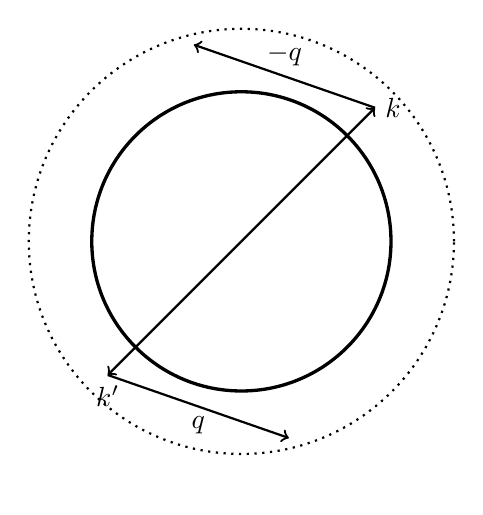
\begin{tikzpicture}
        \coordinate (a) at (1.697, 1.697);
        \coordinate (b) at (-1.697, -1.697);
        \coordinate (shift) at (0,-3);
        \filldraw[color=black, fill = white!0 , thick, dotted](0,0) circle (2.7);
        \filldraw[color=black, fill = white!0, very thick](0,0) circle (1.9);
        \draw[->, thick] (0,0) -- (a) node[anchor = west]{$\bm{k}$};
        \draw[->, thick] (0,0) -- (b) node[anchor = north]{$\bm{k}'$};
        \draw[->, thick] (a) -- ++(-2.3,0.8) node[midway, anchor = south]{$-\bm{q}$};
        \draw[->, thick] (b) -- ++(2.3,-0.8) node[midway, anchor = north]{$\bm{q}$};
        \filldraw[color=white, fill = white!0 , thick, dotted] (shift) circle (0.1);3
    \end{tikzpicture}
    \caption{The scattering process of two electrons with opposite wavevectors $\bm{k}$ and $\bm{k}'$. We have a momentum transfert $\bm{q}$ between them. 
    The thick line illustrates the Fermi-surface and the dotted one the thin shell. As we see if the electrons have opposite wavevectors, and the $\bm{k}$ electrons
    scatters into the shell, then the $\bm{k}'$ electron scatters in the shell as well. This is not allways the case if the wavevectors don't agree as we can see on the left figure.
    The right figure points out the maximisation process. With opposite wavevectors,
    we get the largest possbility spectrum for the scattering.}
\end{figure}
Further the attractivity is a short range effect, so if we want to consider it, we must think that the electrons are very close to eachother.
This requires the electrons to have opposite spins due to the Pauli principle. This is a same as a lattice site. This is the only 
possbility for them to cohabit the same neighbourhood. \rem{check} The approximation turns out to be a good model.\\

Now we allow us to rename some variables:
\[
    \bm{k} + \bm{q} \longrightarrow \bm{k} ~,~~ \bm{k} \longrightarrow \bm{k}'
\]
The Hamiltonian that follows from these transformations is called the BCS-reduced Hamiltonian
\begin{equation} \label{eq:BCS_ReducedHamiltonian}
    H = \sum_{\bm{k},\sigma} \epsilon_{\bm{k}} c_{\bm{k},\sigma}^{\dagger}c_{\bm{k},\sigma} + \sum_{\bm{k},\sigma,\bm{k}} V_{\bm{k}\bm{k}'} c_{\bm{k},\sigma}^{\dagger}c_{-\bm{k},-\sigma}^{\dagger}c_{-\bm{k}',-\sigma}c_{\bm{k}',\sigma}
\end{equation}
$V_{\bm{k}\bm{k}'}$ is now a matrix element that acts if the wavevectors are close to the Fermi-surface. The electrons have to move in opposite directions with opposite spins.
Due to the retardation processes we introduced earlier, there remains a distortion in the lattice long after the electrons passed. Due to the inducting dipol moment,
the other electron is attracted towards the distortion with $M_{\bm{q}}$ \rem{?}. As we also saw, the coulomb repulsion causes a colinear displacement, close to the distortion
of the homologue. This phenomenon is called the Cooper-pairing and is a coupling that happens in momentum space.\\

An interacting fact is that these interactions are the source of the superconductivity but they are also to main origin of resistivity in clean materials.

\subsection{On our way to the BCS-theory}
After this introduction on the phonon coupling between the electrons in the momentum space, or Cooper-pairing,
we aim to describe the energy of the superconductor in a mean-field approach. The goal of it is to reduce the description
with the neighbours to the description of a site, in the mean field of the other sites. Thefore we are going to describe 
a one-boby problem which is easier to compute. As known mean-fiels approches requier self-consistent equations that will as well follow.\\

The first step is to introduce the following epexctation values:
\begin{align}
    b_{\bm{k}} = &\langle c_{-\bm{k}\downarrow}c_{\bm{k}\uparrow}\rangle \label{eq:ExpectBCS} \\
    b_{\bm{k}}^{\dagger} = &\langle c_{\bm{k}\uparrow}^{\dagger}c_{-\bm{k}\downarrow}^{\dagger}\rangle  \label{eq:ExpectBCSDag}
\end{align}
wich lead to a new expression for the $c$ operators:
\begin{equation}
    c_{-\bm{k}\downarrow}c_{\bm{k}\uparrow} = b_{\bm{k}} + \underbrace{c_{-\bm{k}\downarrow}c_{\bm{k}\uparrow} - b_{\bm{k}}}_{\delta_{b_{\bm{k}}}}
\end{equation}
where we can see the $\delta_{b_{\bm{k}}}$ as a deviation, or fluctuation term. If we introduce it back into the Hamiltonian, we can write
\[
    H = \sum_{\bm{k}\sigma} \epsilon_{\bm{k}} c_{\bm{k}\sigma}^{\dagger}c_{\bm{k}\sigma} + \sum_{\bm{k},\bm{k}'} V_{\bm{k}\bm{k}'} \bigl( b_{\bm{k}}^{\dagger} + \delta_{b_{\bm{k}}}^{\dagger}\bigr)\bigl( b_{\bm{k}} + \delta_{b_{\bm{k}}}\bigr).
\]
We can compute the product of the two terms in parenthesis and forget the $\mathcal{O}\left(\delta_{b_{\bm{k}}}^2\right)$ because the fluctuation are small. We then obtain the following expression
\[
    H = \sum_{\bm{k}\sigma} \epsilon_{\bm{k}} c_{\bm{k}\sigma}^{\dagger}c_{\bm{k}\sigma} + \sum_{\bm{k},\bm{k}'} V_{\bm{k}\bm{k}'} \left( b_{\bm{k}}^{\dagger}c_{-\bm{k}'\downarrow}c_{\bm{k}'\uparrow}  + b_{\bm{k}'}^{\dagger} c_{\bm{k}\uparrow} ^{\dagger}c_{-\bm{k}\downarrow}^{\dagger} -  b_{\bm{k}}^{\dagger} b_{\bm{k}'}\right).
\]

The next step is to define the superconduction gap parameter $\Delta$:
\begin{align}
    \Delta_{\bm{k}} = &\sum_{\bm{k}'} V_{\bm{k}\bm{k}'} b_{\bm{k}}^{\dagger}\\
    \Delta^{\dagger}_{\bm{k}} = &\sum_{\bm{k}'} V_{\bm{k}\bm{k}'} b_{\bm{k}'}
\end{align}
wich brings our Hamiltonian in another form:
\begin{equation} \label{eq:HamiltonianBCS1}
    H = \sum_{\bm{k}\sigma} \epsilon_{\bm{k}} c_{\bm{k}\sigma}^{\dagger}c_{\bm{k}\sigma} - \sum_{\bm{k}} \left( \Delta_{\bm{k}}^{\dagger} c_{-\bm{k}'\downarrow}c_{\bm{k}'\uparrow}  + \Delta_{\bm{k}}^{\dagger} c_{\bm{k}\uparrow} ^{\dagger}c_{-\bm{k}\downarrow}^{\dagger} -  b_{\bm{k}}^{\dagger} \Delta_{\bm{k}}^{\dagger} \right).
\end{equation}
We took the liberty to spilt the sum, rename the $\bm{k}'$ to $\bm{k}$ and recombine the sum. We notice that this form involves a lot of creation and annihilation terms that 
are not commun for an effective non-interacting electron gaz. We remeber that we aim a one particle descirption in a mean field of its neighbours.
This complexity will lead to some difficulties to express the quais-particle spectrum. A good soltution is 
to rotate the basis of the $c$ operators to land in a basis that diagonalises the Hamiltonian and therfore minimises the number of operators.\\

The transformation involves two new fermionic operator $\eta$ and $\gamma$ that therfore respect \ref{eq:Fermion1} to \ref{eq:Fermion3} and reads
\begin{equation*}
    \begin{pmatrix}
        c_{\bm{k}\uparrow}\\
        c_{-\bm{k}\downarrow}^{\dagger}
    \end{pmatrix} = 
    \begin{pmatrix}
        \cos(\theta) & -\sin(\theta)\\
        \sin(\theta) & \cos(\theta)
    \end{pmatrix}
    \begin{pmatrix}
        \eta_{\bm{k}}\\
        \gamma_{\bm{k}}
    \end{pmatrix}
\end{equation*}
along with the conjugate transpose of each component of the l.h.s vector rebuild into a matrix-vector equation
\begin{equation*}
    \begin{pmatrix}
        c_{\bm{k}\uparrow}^{\dagger} \\
        c_{-\bm{k}\downarrow}
    \end{pmatrix} = 
    \begin{pmatrix}
        \cos(\theta) & -\sin(\theta)\\
        \sin(\theta) & \cos(\theta)
    \end{pmatrix}
    \begin{pmatrix}
        \eta_{\bm{k}}^{\dagger} \\
        \gamma_{\bm{k}}^{\dagger}
    \end{pmatrix}.
\end{equation*}
We can reintroduce these into the Hamiltonian \ref{eq:HamiltonianBCS1}. 
Some of the multiplication involves $\cos(\theta)^2 - \sin(\theta)^2 = \cos(2\theta)$ and $\cos(\theta)^2 + \sin(\theta)^2 = 1$. 
Further due to the anticommutations we have $\eta \gamma^{\dagger} = - \gamma^{\dagger}\eta$ and so on for $\gamma \eta^{\dagger} = - \eta^{\dagger}\gamma$.
We obtain the following expression
\begin{equation}
    \begin{aligned}
        H =& \sum_{\bm{k}} \epsilon_{\bm{k}}\rem{\cdot 1} + \Delta_{\bm{k}}b_{\bm{k}}^{\dagger}\\
          +& \sum_{\bm{k}} \left[\epsilon_{\bm{k}}\cos(2\theta) - \cos(\theta)\sin(\theta)\left(\Delta_{\bm{k}}^{\dagger}+ \Delta_{\bm{k}}\right)\right] \eta_{\bm{k}}^{\dagger}\eta_{\bm{k}}\\
          -& \sum_{\bm{k}} \left[\epsilon_{\bm{k}}\cos(2\theta) -\sin(\theta)\cos(\theta)\left(\Delta_{\bm{k}}^{\dagger}+ \Delta_{\bm{k}}\right)\right]\gamma^{\dagger}_{\bm{k}}\eta_{\bm{k}}\\
          -& \sum_{\bm{k}} \left[\Delta_{\bm{k}} \cos(\theta)^2 - \Delta_{\bm{k}}^{\dagger}\sin(\theta)^2 \rem{+}2\epsilon_{\bm{k}} \cos(\theta)\sin(\theta) \right]\eta^{\dagger}_{\bm{k}}\gamma_{\bm{k}}\\
          -& \sum_{\bm{k}} \left[\Delta_{\bm{k}} \cos(\theta)^2 - \Delta_{\bm{k}}^{\dagger}\sin(\theta)^2 \rem{+}2\epsilon_{\bm{k}} \cos(\theta)\sin(\theta) \right]\gamma^{\dagger}_{\bm{k}}\eta_{\bm{k}}.     
    \end{aligned}
\end{equation}
The goal is to diagonalise the Hamiltonian in the $(\gamma, \eta)$ basis. Thefore have to rotate with $\theta$ such that the terms with $\gamma^{\dagger}\eta$ and $\eta^{\dagger}\gamma$ vanish.
A difficulty that we may entcounter along with this idea is that $\Delta$ is an order parameter and own a complex phase fluctuation. With other words one can write
$\Delta = |\Delta|e^{\im\tau}$ where $\tau$ has has some fluctuations. We are going to ignore them.\\

We can set
\[
    \Delta_{\bm{k}} = \Delta_{\bm{k}}^{\dagger}~~~~ \text{and} ~~~~ \tan(2\theta) = -\frac{\Delta_{\bm{k}}}{\epsilon_{\bm{k}}}
\]
and introduce two new variables called the coherence factors
\begin{align*}
    v_{\bm{k}}^2 := \sin(\theta)^2 &= \frac{1}{2} \left(1 - \frac{\epsilon_{\bm{k}}}{E_{\bm{k}}}\right),\\
    u_{\bm{k}}^2 := \cos(\theta)^2 &= \frac{1}{2} \left(1 + \frac{\epsilon_{\bm{k}}}{E_{\bm{k}}}\right)
\end{align*}
along with a new energy $E_{\bm{k}} = \sqrt{\epsilon_{\bm{k}}^2 + |\Delta_{\bm{k}}|^2}$. \rem{Historical context?} These factors play an important
role in NMR as well as in the ultra sound propagation in superconductors. Cooper and Schrieffer made some corrrect
predictions in an advanced many-body system. This is labeld as one of the greates achievements in condensed matter physics in the 20th century.\\ \rem{source}

We obtain a Hamiltonian that looks very similar to a free fermion qusiparticle gas \rem{source?}
\[
H = \underbrace{\sum_{\bm{k}} \left(\epsilon_{\bm{k}} + \Delta_{\bm{k}} b_{\bm{k}}^{\dagger}\right)}_{\substack{=:H_0~ \text{constant}\\\text{ mean-field term}}}  + \underbrace{\sum_{\bm{k}} E_{\bm{k}}\left(\eta_{\bm{k}}^{\dagger}\eta_{\bm{k}} - \gamma_{\bm{k}}^{\dagger}\gamma_{\bm{k}}\right)}_{\substack{\text{Spinless fermion system with} \\\text{two types of fermions of}\\\text{energies }E_{\bm{k}}\text{ and }-E_{\bm{k}}.}}.
\]
where we dont describe any interaction, but two types of particles in a mean field. One can also note that we don't have any spins involved. This is due
to the fact that we describe the quasiparticles as a linear combiantion of electrons and holes with opposite spins. \rem{source}
Therfore talking about degrees of freedom the two electron-hole singlets replace the $\uparrow$, $\downarrow$ degrees of freedom and they are preserved.\\

The ernegy $E_{\bm{k}}$ shows up a gap in the energy of the qusiparticle whene looking at the fermi-surface $\epsilon_{\bm{k}}=0$ \rem{We count relative to it? But the way it is define in a non interacting Ham. is not relative to it right?}.
This is due to the fact that the exepectation values we introduced in \ref{eq:ExpectBCS} and \ref{eq:ExpectBCSDag} are not zero. The gap is a result of the Cooper-pairing. These expections values
are the order parameters of the Meissner state and should be confused with the superconducting gap $\Delta$. They are however zero at the same time. \rem{source?}\\
\end{document}

